\scanpage{11}
étant soumis à une condition de transitivité pour un composé \(v_{\unsure{\circ|o}}u\) de flèches de \(S\) , et à la condition que \(u\varepsilon\underline{M}\) implique que \(\handwritten{\varphi}_u\) soit un isomorphisme .

\handwritten{3}) Définir des foncteurs ``restrictions '' et `` prolongement ''
\[
\operatorname{Res}_X:(S_{\handwritten{/}X})^{\handwritten{\sim}}\to S(X)^{\handwritten{\vee}}\ ,\quad
\operatorname{Prol}_X:S(X)^{\handwritten{\sim}}\to(S_{\handwritten{/}X})^{\handwritten{\sim}}\ ;
\]
montrer que \(\operatorname{Res}_X\) commute aux limites inductives et aux limites projectives et que \(\operatorname{Prol}_X\) est \uline{pleinement fidèle} , son image essentielle étant formée des faisceaux \(F\) tels que \(\handwritten{\varphi}_u\) soit un isomorp\unsure{\deleted{g}h|\deleted{h}g}isme pour toute flèche \(u\) de \deleted{du} \(S_{\handwritten{/}X}\) .

\handwritten{4}) Définir un isomorphisme d'adjonction faisant de \(\operatorname{Res}_X\) l'adjoint à droite de \(\operatorname{Prol}_X\) . En conclure qu'il existe un morphisme de topos
\[
f:S(X)^{\handwritten{\sim}}\to(S_{\handwritten{/}X})^{\handwritten{\sim}}
\]
tel que \(f^{\handwritten{*}}=\operatorname{Res}_X\) et que le foncteur \(f^{\handwritten{*}}\) admet un adjoint à gauche \(f_!=\operatorname{Prol}_X\) . Montrer que \(\operatorname{Prol}_X\) transforme les faisceaux abéliens en faisceaux abéliens . Montrer que \(f:S(X)^{\handwritten{\sim}}\handwritten{\longrightarrow}(S_{\handwritten{/}X})^{\handwritten{\sim}}\) est un \uline{plongement} de topos (\handwritten{9}.\handwritten{1}.\handwritten{1}) et que par suite ``le petit topos '' \(\handwritten{S(X)^{\sim}}\) est \deleted{un sous-topos \unsure{(9.1}} équivalent à un sous-topos du ``gros topos '' \((S_{\handwritten{/}X})^{\handwritten{\sim}}=S^{\handwritten{\sim}}_{\handwritten{/}X}\) .

\handwritten{5}) Soit \(F\) un faisceau abélien flasque de \(S^{\handwritten{\sim}}_{\handwritten{/}X}\) (V \handwritten{4}) . M\textsuperscript{O}ntrer que \(\operatorname{Res}_X F\) est \(S(X)\)-acyclique\handwritten{\begin{tikzpicture}[baseline=-0.6ex,x=1ex,y=1ex]\draw[line width=.45pt] (0,-.55) -- (.52,2.05) .. controls (.86,2.27) and (.86,2.67) .. (.60,2.63) .. controls (.34,2.55) and (.42,2.16) .. (.52,2.05);\end{tikzpicture}}\reversemarginpar\margin{\handwritten{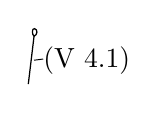
\begin{tikzpicture}[baseline=0ex,x=1ex,y=1ex]\draw[line width=.45pt] (0,-1.2) -- (.48,2.8) .. controls (.80,2.95) and (.79,3.4) .. (.53,3.45) .. controls (.27,3.48) and (.31,2.97) .. (.48,2.8);\draw[line width=.35pt] (.48,.8) -- (1.25,.9);\node[anchor=west,inner sep=0pt] at (1.22,.8) {\inserted{(V 4.1)}};\end{tikzpicture}}}\normalmarginpar . En déduire que pour tout faisceau abélien \(F\) de \(S^{\handwritten{\sim}}_{\handwritten{/}X}\) et tout entier \(q\) , le groupe \(H^q(X,F)\) (cohomologie calculée dans \(S^{\handwritten{\sim}}_{\handwritten{/}X}\) ) est canoniquement isomorphe au groupe \(H^q(X,\operatorname{Res}_X F)\) (cohomologie calculée dans \(S(X)^{\handwritten{\sim}}\) ) .

\handwritten{6}) Déduire de 5) que pour tout faisceau abélien \(G\) \deleted{sur} de \(S(X)^{\handwritten{\sim}}\) et tout entier \(q\) le groupe \(H^q(X,G)\) \deleted{(resp.} (cohomologie calculée dans \(S(X)^{\handwritten{\sim}}\) ) est canoniquement isomorphe aux groupes \(H^q(X,f_{\handwritten{*}}G)\) et \(H^q(X,\operatorname{Prol}_X G)\) (cohomologie calculée dans \(S^{\handwritten{\sim}}_{\handwritten{/}X}\) ) .
% archive sheet number: 10
